\section{Koncept identifikace nejlepší nosnice}\label{sec:koncept-identifikace-nejlepsi-nosnice}

Při chovu slepic by bylo velmi užitečné vědět, kolik vajec která slepice snáší, protože to umožňuje farmáři sledovat produktivitu jednotlivých slepic.
Díky tomu může:
\begin{itemize}
    \item Optimalizovat chov: Identifikací slepic s vysokou a nízkou snáškou může farmář rozhodnout o selekci nebo o zvláštní péči pro méně produktivní slepice.
    \item Zlepšit zdraví slepic: Nízká snáška může být indikátorem zdravotních problémů.
    Včasná identifikace umožňuje podniknout kroky k léčbě nebo prevenci nemocí.
    \item Efektivněji plánovat krmení a zdroje: Sledování výkonu pomáhá v rozhodování o výživě a péči, aby byla maximalizována produkce vajec při optimálních nákladech.
    \item Zvýšit ziskovost: Monitorováním snášky lze zlepšit celkovou produktivitu farmy a tím i její ekonomickou efektivitu.
\end{itemize}

Obecně můžeme říci, že znalost počtu snesených vajec od každé slepice pomáhá v efektivním řízení chovu a zajišťuje lepší výsledky jak po stránce produkční, tak ekonomické.

Abych toho dosáhl, potřebuji být schopen jednotlivé slepice identifikovat a tuto informaci propojit s momentem, kdy slepice snese v hnízdě vejce.
V sekci~\ref{sec:digitalni-vaha-do-hnizda}, je popsan mechanismus, kdy pravidelnou analyzou casove rady, kterou poskytuje vaha ziskame informaci o casove udaji, kdy bylo vejce sneseno.
Pak jiz jen staci identifikovat, ktera z nasich slepic byla v tu dobu v hnízdě.

Existuje několik variant, jak slepice identifikovat, já jsem se rozhodl využít k identifikaci obrazovou analýzu.
Vždycky mě zajímalo na jakém principu funguje rozpoznávání lidí na základě kamerových záznamů, které používá policíe případně sledování vozidla, které projíždí nočním městem na červenou skze několik křižovatek.

Hledání zdrojů na internetu mě přivedlo ke spoustě článků, příspěvků, příkladů i vědeckých prací.

Nakonec jsem nalezl článek \cite{medium-person-reidentification}, který mě inspiroval.

Z článku jsem pochopil zakladní princip.

Postupuji následujícím způsobem.
Nejprve procházím videozáznam a identifikuji oblasti, kde se slepice nacházejí.
Tyto oblasti následně vystřihnu a uložím do samostatných souborů.
Poté procházím tyto menší obrázky a pomocí segmentace vystřihnu plochu, kde je slepice, zatímco ostatní části zůstanou bílé.
Takto vyříznuté obrázky převádím na tenzory.
Převod na tenzor znamená, že dvourozměrný obraz (matice pixelů) převedu do vícerozměrné datové struktury, která dokáže reprezentovat různé vlastnosti obrazu a je vhodná pro strojové učení a další matematické zpracování.
Tímto způsobem získám numerickou reprezentaci obrazu, se kterou mohu efektivně pracovat.
Získané tenzory porovnávám se vzorovými vektory uloženými v databázi.
Pokud je vektor shodný, znamená to, že jsem našel odpovídající slepici, a podařilo se mi ji tak identifikovat.

Algoritmus tedy na počátku vezme jako vstup obrázek z kamery viz obrázek~\ref{fig:source_chick_image}.

\begin{figure}[H]
    \centering
    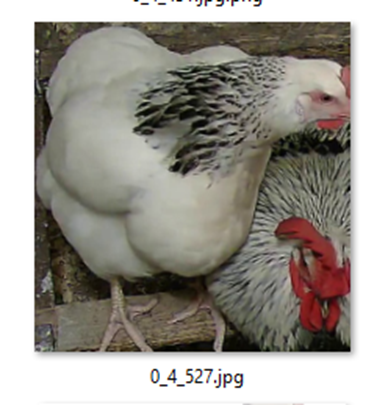
\includegraphics[width=0.3\textwidth]{img/source_chick_image}
    \caption{Jeden ze vstupů do algoritmu pro nosnice}
    \label{fig:source_chick_image}
\end{figure}

Dále je slepice z obrázku vystřižena (segmentována) podle kontury, kterou algoritmus vyhodnotil jako slepice viz obrázek~\ref{fig:segmented_chicks2}.

\begin{figure}[H]
    \centering
    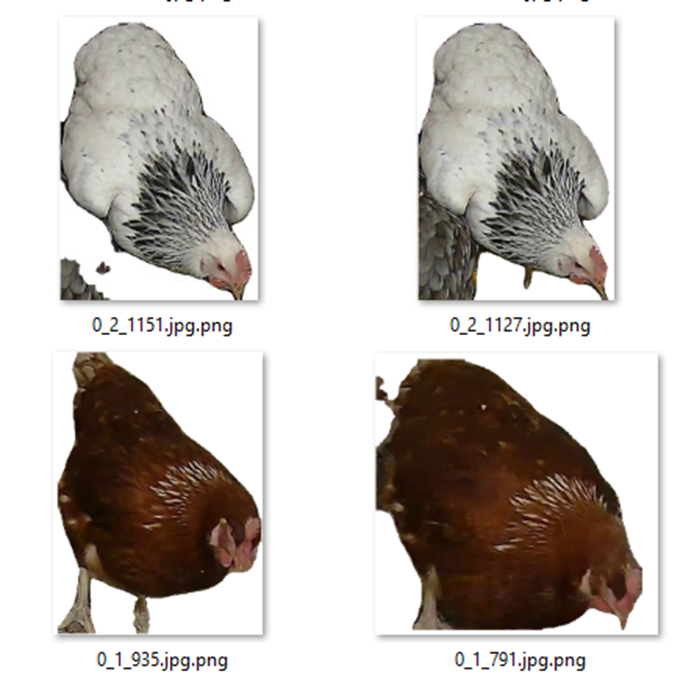
\includegraphics[width=0.3\textwidth]{img/segmented_chicks}
    \caption{Segmentované slepice z fotek}
    \label{fig:segmented_chicks2}
\end{figure}

Na závěr je pro každý výřez vypočítán tenzor na jehož základě jsou slepice roztřízeny do jednotlivých skupin viz obrázek~\ref{fig:chicks_in_clusters}.

\begin{figure}[H]
    \centering
    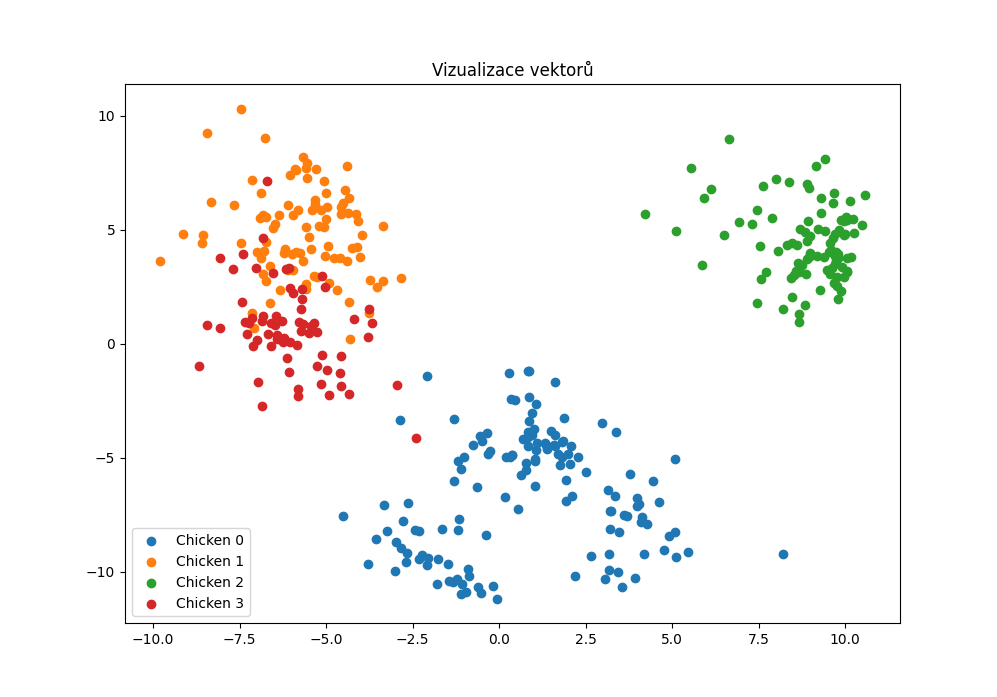
\includegraphics[width=0.3\textwidth]{img/chicks_in_clusters}
    \caption{Algoritmem rozdělené slepice dle tenzorů}
    \label{fig:chicks_in_clusters}
\end{figure}
\begin{figure}[h]
    \centering
    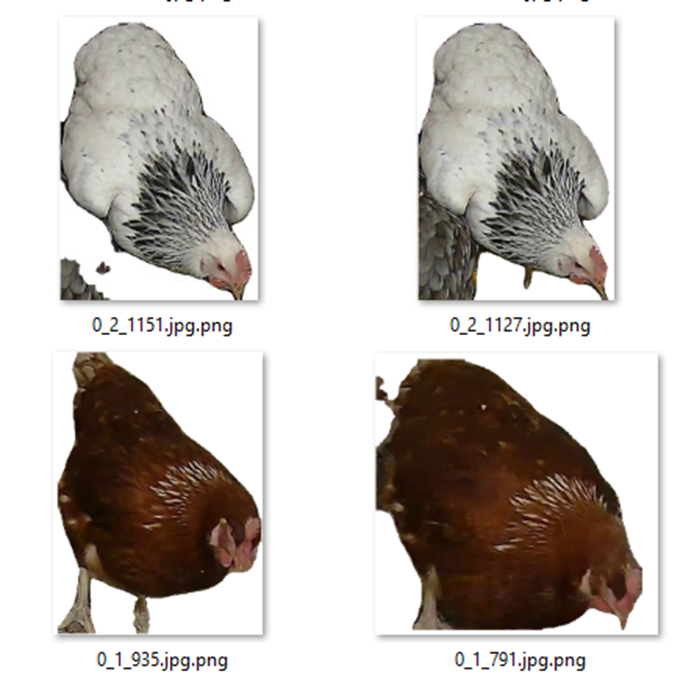
\includegraphics[width=\textwidth]{img/segmented_chicks}
    \caption{Segmentované slepice z fotek}
    \label{fig:segmented_chicks}
\end{figure}


Zmiňuji tuto funkcionalitu v sekci "plány do budoucna", protože se mi zatím nepodařilo algoritmus dostatečně vypilovat.
Při vývoji jsem sice testoval na několika obrázcích a zdálo se, že princip by mohl fungovat, ale v reálném prostředí byl výsledek značně nepřesný.
Babička má totiž dvakrát červenou, dvakrát bílou a dvakrát černou slepici, plus jednoho bílého kohouta.
Proto jsou ty slepice často hodně podobné a rozdíly mezi nimi jen nepatrné.

Momentálně přemýšlím, jak ty slepice odlišit, ale nejsem si jistý, že by mi babička dovolila je pomalovat.
Možná by pomohlo i zjednodušení úkolu.
Namísto soutěže o nejlepší nosnici bych se možná mohl zamyslet nad sestavením nejlepšího závodního týmu.

Mohly by to být týmy bílých, červených či černých slepic.





